% !TeX spellcheck = de_DE
\documentclass[a4paper,11pt,singlespacing]{article}

\usepackage{setspace}
\usepackage[utf8]{inputenc}
\usepackage[T1]{fontenc}
\usepackage{graphicx}
\usepackage{color}
\usepackage{hyperref}
\usepackage{listings,xcolor}
\usepackage{pdfpages}
\usepackage{float}

\renewcommand{\figurename}{Abbildung}

\graphicspath{ {./images/} }

\begin{document}
	\setlength{\parindent}{0ex}
	
	\begin{titlepage}
		\author{Luca Asmus\\ Marius Würstle\\Rolf Wiersch}
		\title{
\includegraphics[scale=0.3]{rwu_logo_hor-lila-cyan_rgb_0} \\ ~\\ ~\\ WLAN-AP mit regelmäßigem PSK-Tausch und QR-Code Anmeldung \vspace{8cm}}
		\date{\today}
		\maketitle
		\thispagestyle{empty}
    	\end{titlepage}
    	
    	\section{Zusammenfassung}
    	Das Ziel dieses Projekts war es, die Sicherheit im eigenen Gast-WLAN zu gewährleisten, unter Berücksichtigung der Faulheit und Bequemlichkeit vieler Endnutzer. Der pre-shared Key eines WLANs wird in den meisten Netzwerken einmal oder nie geändert. Dadurch können Gäste dauerhaften Zugang zum Netzwerk behalten, obwohl das nicht erwünscht ist. Ein weiteres Problem ist die Umständlichkeit einen sicheren pre-shared Key zu verwenden. Es führt zu unangenehmen Mehraufwand eine kryptische und lange Zeichenkette auf Endgeräten einzugeben. Gelöst wurde dies durch einen eigenen Access Point für Gäste. Über diesen wird der Zugriff ins Internet geleitet. Der pre-shared Key wird einmal die Woche oder manuell neu erzeugt und auf einem Display ausgegeben. Die Ausgabe erfolgt in Form eines QR - Codes und in Klartext.   \\

    	
    	
    	\tableofcontents
    	\newpage
    	
    	\section{Abbildungsverzeichnis}
    	\listoffigures
    	\newpage
    	
    	\section{Allgemeines}
    	
    	\subsection{Fachbegriffe}
    	host access point daemon = hostapd
    	sed = Stream EDitor, Unix-Werkzeug zum Bearbeiten von Text
    	stdout = Standard Ausgabe, normalerweise mit Monitor verbunden
    	
      	\section{Hardware}
    		\subsection{Raspberry Pi}
    			Der Raspberry Pi wurde für junge Menschen entwickelt, um ihnen eine preisgünstige Möglichkeit zu bieten, sich mit der Informatik zu beschäftigen. Der Einplatinencomputer ist etwa kreditkartengroß und kam Anfang 2012 auf den Markt. Er ermöglicht einen schnellen und praktischen Weg um Wissen in den Bereichen Programmieren und Hardware zu erlangen. Zudem ist er vielseitig einsetzbar, in diesem Fall wird er zu einem Access-Point konfiguriert. 
    			\begin{figure}[H]
    				\centering
	    			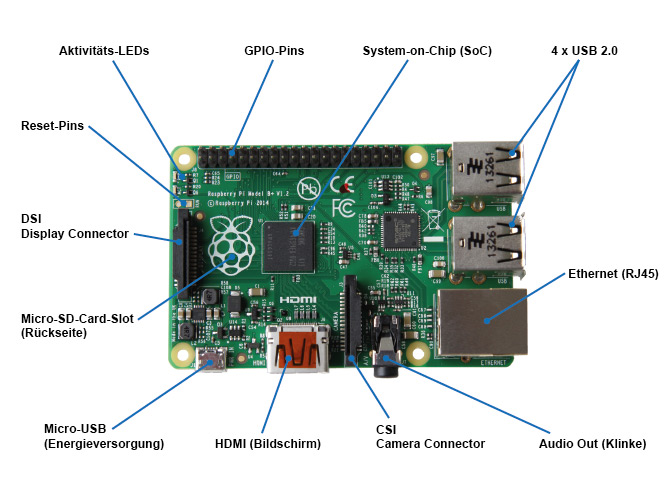
\includegraphics[scale=0.5]{raspberry_pi_3b}
	    				\caption{Raspberry Pi 3b - Quelle: \cite{Picture_Raspberrypi3b} }
	    				\label{raspberrypi3b}
				\end{figure}
				Technische Spezifikationen unseres Raspberry Pi 3b:
				\begin{itemize}
					\item Quad Core 1.2GHz Broadcom BCM2837 64bit CPU
					\item 1GB RAM
					\item BCM43438 wireless LAN and Bluetooth Low Energy (BLE) on board
					\item 100 Base Ethernet
					\item 40-pin extended GPIO
					\item 4 USB 2 ports
					\item 4 Pole stereo output and composite video port
					\item Full size HDMI
					\item CSI camera port for connecting a Raspberry Pi camera
					\item DSI display port for connecting a Raspberry Pi touchscreen display
					\item Micro SD port for loading your operating system and storing data
					\item Upgraded switched Micro USB power source up to 2.5A
				\end{itemize}
			\subsection{Raspberry Pi Shield - Display LCD-Touch, 3,2in}
				Der Touchscreen wertet den Raspberry Pi zu einem vollwertigen Touch-PC auf. Für zusätzliche Funktionen besitzt der Display 3 Buttons an der Seite, welche einfach über die GPIO Pins eingelesen werden können.
				\begin{figure}[H]
					\centering
					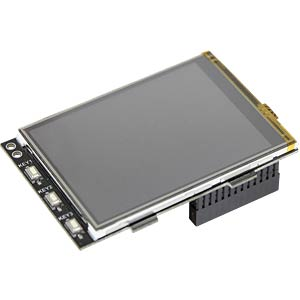
\includegraphics[scale=0.5]{touch_display}
					\caption{Touchscreen Display für den Raspberry Pi - Quelle: \cite{Picture_touchdisplay}}
					\label{touchdisplay}
				\end{figure}
				Technische Spezifikationen unseres Raspberry Pi Shield - Display LCD-Touch, 3.2in:
				\begin{itemize}
					\item Display 8,13cm (3,2")
					\item Auflösung 320 x 240 Pixel
					\item LED-Hintergrundbeleuchtung
					\item 3 frei belegbare Taster (angebunden an GPIO12, 16, 18)
					\item SPI-Schnittstelle
					\item Touchscreen Technologie resistiv
				\end{itemize}
			\subsection{SD-Karte}
    			Die SD-Karte ist eine SanDisk extreme mit einer Speicherkapazität von 32GB. Sie dient als Speichermedium des Raspberry Pi's. Zu Beginn wird das Betriebssystem auf die Karte geflasht von dieser wird der Einplatinencomputer gebooted.

    			
    	\section{Software}
    		\subsection{balenaEtcher}
    			Flash Sd Card
    		\subsection{hostapd}
        		Mit hostapd ist es möglich Geräte, die ein WLAN-Modul besitzen, als Access Point zu betreiben. Jedoch können keine Einstellungen im Bereich IP und Routing vorgenommen werden. Die Software ist nur für das Erstellen eines "wireless Ethernet switches" zuständig. \cite{Quote_hostapd1} 
    		\subsection{dnsmasq}
        		Geräte in einem Netzwerk benötigen zur Kommunikation eine IP Adresse und einen DNS Server für die Namensauflösung. Deshalb muss in diesem Projekt ein DHCP und DNS erstellt werden. Von diesen bekommen die Endgeräte ihre IP Konfiguration im WLAN. Die Software dnsmasq wird in diesem Projekt verwendet, um dies zu ermöglichen.
    		\subsubsection{netfilter-persistent und iptables-persistent}
        		Für die Durchführung des Projektes ist es nötig iptables-Regeln anzulegen. Diese sollten nach einem Neustart nicht neu angelegt werden müssen. Deshalb wurden die Pakete netfilter-persistent und iptables-persistent installiert. Damit können die Regeln in eine Datei abgespeichert und beim Neustart automatisch geladen werden.
        	\subsection{Bash}
        		Im Projekt wird Bash benutzt um die einzelnen Python Skripte aufzurufen, Infos aus Konfigurationsdateien auszulesen und schnelle Änderungen an Diesen vorzunehmen. Bash ist als Standardshell bei Raspberry Pi OS Lite vorinstalliert. 
    		\subsection{Cron}
				Cron ermöglicht das zeitbasierte Ausführen des Bash Skripts. So kann beispielsweise jeden Montag um 03:00 Uhr nachts das Passwort automatisch geändert werden. 
    		\subsection{Python 3.7}
    			Für die Skripte zur Passwortgenerierung, QR-Code Generierung und zum Einlesen der Buttons wird die Sprache Python verwendet. Python 3.7 ist bei Raspberry Pi OS Lite  vorinstalliert und erleichtert durch verschiedene Bibliotheken die Umsetzung des Projektes.
    			\subsubsection{pyqrcode}
    				Das Modul pyqrcode wird dafür benutzt, möglichst einfach und frei QR-Codes zu erzeugen. Zum Erzeugen des Codes benötigt sie nur die Parameter die enthalten sein sollen.
    			\subsubsection{gpiozero}
    				Im Beta-Stand noch nicht umgesetzt
    	
    	\section{Vorbereitung des Raspberry Pi}
    	\subsection{Auswahl und Installation des Betriebssystem}
    	    Um mit dem Projekt beginnen zu können musste zuerst ein Betriebssystem bestimmt werden.
        	Es wurde sich für das Raspberry Pi OS Lite entschieden. Begründet wurde diese Entscheidung  durch die weniger vorinstallierten Pakete und einer fehlender grafischen Bedienoberfläche. Hierdurch konnte Speicherplatz und Sicherheitsrisiken eingespart werden. Je weniger unbenutzte Software, desto weniger Angriffsfläche. \\ 
    	
        	Nach der Auswahl des Betriebssystems konnte dieses auf eine SD-Karte geschrieben werden.
        	Hierzu wurde die Software balenaEtcher verwendet.   
    	
    	
    	\subsection{Aktualisierung und Paketinstallation}
        	Nach der Neuinstallation eines Betriebssystems fehlen diesem oft die aktuellsten Versionen von Softwarepaketen und Updates. Deshalb wurden diese zuerst aktualisiert und installiert. So werden Konflikte aufgrund veralteter Software vermieden und die Sicherheit verbessert.  
        	Darauf folgte das Nachinstallieren der für das Projekt noch benötigten Pakete. Diese wurden im Abschnitt Software genauer beschrieben. 
    	
    	
    	\subsection{SSH Zugriff einrichten}
    	Da das Projektteam aus drei Personen besteht, wurde ein SSH Zugriff in den Einstellungen des Raspberry Pi eingerichtet. Die Einstellungen können mit folgendem Befehl geöffnet werden: 
    	\lstset{
        language=bash,
        keywordstyle=\color{blue},
        commentstyle=\color {violet},
        stringstyle=\color{orange},
        numbers=left,
        basicstyle=\scriptsize\ttfamily,
        showspaces=false,
        frame= single,
        xleftmargin=0.5cm
        }
        \begin{lstlisting}
sudo raspi-config
        \end{lstlisting} 
    	
        In diesem Zuge wurde der SSH Zugriff aktiviert und das Standardpasswort geändert. Durch den  Zugriff konnte das parallele Arbeiten am Projekt ermöglicht werden. 
    	\section{Konfiguration des RaspberryPi als funktionalen Access-Point}
            \subsection{WLAN Interface}
                Der Raspberry Pi benötigt eine statische IP Konfiguration für sein WLAN Interface. Diese wird in der Datei /etc/dhcpcd.conf vorgenommen. Die Datei wird um folgendes ergänzt:\\
                \lstset{
                language=bash,
                }
                \begin{lstlisting}
interface wlan0
    static ip_address=192.168.4.1/24
    nohook wpa_supplicant
                \end{lstlisting} 
                Mit der 192.168.4.1 wird eine statische IP Adresse vergeben unter die der Raspberry Pi im WLAN erreichbar ist. Weiterhin wird der wpa{\_}supplicant deaktiviert um keine Konflikte mit hostapd zu verursachen. 
            
            \subsection{Routing}
                Der Access Point muss den Datenverkehr der Endgeräte im WLAN zum Router weiterleiten können.
                Hierzu wird in /etc/sysctl.d/routed-ap.conf ein Eintrag hinzugefügt bzw. das Kommentarzeichen entfernt:\\
                \lstset{
                language=bash,
                }

                \begin{lstlisting}
# Enable IPv4 routing
net.ipv4.ip_forward=1
                \end{lstlisting} 
                Endgeräte können nun den Hauptrouter erreichen. Um jedoch eine Kommunikation zu ermöglichen muss NAT eingestellt werden. Die wird durch einen Eintrag in die iptables Firewall erreicht: \\
            
                \begin{lstlisting}
sudo iptables -t nat -A POSTROUTING -o eth0 -j MASQUERADE
                \end{lstlisting} 
       
                Bei Datenverkehr zum Hauptrouter wird nun die Absender IP Adresse der Endgeräte mit der IP der LAN-Schnittstelle ersetzt. Bei Rückantworten an den Raspberry Pi werden diese an den jeweiligen Absender richtig weitergeleitet.\\
            
                Um die Firewall Regel bei einem Neustart zu behalten, wurde diese abgespeichert:\\
                
                \begin{lstlisting}
sudo netfilter-persistent save
                \end{lstlisting}    
            \subsection{DNS und DHCP}
                Durch dnsmasq können nun die DHCP und DNS Einstellungen erfolgen. Diese werden in der /etc/dnsmasq.conf Datei vorgenommen. Diese dient als Vorlage und gibt Erklärungen zu den Einstellungen. Zur Übersichtlichkeit wurde diese in nsmasq.conf.orig umbenannt und eine neue Datei mit dem ürsprünglichen Namen erzeugt. In der neuen Datei werden nur die getätigten Konfigurationen eingetragen:
            
            
                \begin{lstlisting}
interface=wlan0 # Listening interface
dhcp-range=192.168.4.2,192.168.4.20,255.255.255.0,24h
                # Pool of IP addresses served via DHCP
domain=wlan     # Local wireless DNS domain
address=/gw.wlan/192.168.4.1
                # Alias for this router
                \end{lstlisting}  
                Zuerst wird das Interface angeben, bei den die DHCP/DNS Konfiguration gelten soll. Die ist das schon vorherig erstellte Interface "wlan0". Es wurde sich auf einen DHCP Bereich von 192.168.4.2/24 - 192.168.4.20/24 entschieden. Dieser umfasst 18 IP Adressen, welcher als ausreichend für eine Woche angesehen wird. Die Lease - Zeit wurde auf 24 Stunden eingestellt, da Gäste meist nicht länger als einen Tag anwesend sind.
                Zuletzt wurde eine lokale DNS Domäne und ein Alias für den Access Point eingestellt. Unter diesem Alias ist dieser nun erreichbar.


            \subsection{Access Point Einstellungen}
                Um den Raspberry Pi als Access Point nutzen zu können musste nun hostapd konfiguriert werden. Hierzu wurde zuerst der Dienst aktiviert und so eingestellt das er beim booten gestartet wird:
                  \begin{lstlisting}
                sudo systemctl unmask hostapd
                sudo systemctl enable hostapd
                  \end{lstlisting} 
                
                    Nun musste die Konfigurationsdatei unter /etc/hostapd/hostapd.conf erstellt und gefüllt werden.
                    In dieser werden verschiedene Parameter eingestellt. Darunter fallen unter anderem die SSID, das Passwort und die Art der Verschlüsselung. Es wurde eingestellt das nur WPA2 verwendet wird, da WEP als unsicher gilt. Weiterhin wurde der Funkstandard auf n und 2.4GHz eingestellt. Grund hiefür war das der Raspberry Pi keinen höheren Standard in Form von z.B AC unterstützen würde. Weiterhin ist der eingestellte Standard ausreichend  für das surfen im Gast-Internet. \\
                    Der Kanal wurde auf null gesetzt. Mit dieser Einstellung sucht der Access Point automatisch einen passenden Kanal. Bedeutet, den mit den wenigsten Störungen bzw. einen Kanal der sich möglichst wenig mit anderen Netzen überschneidet.\\
                    Um Wireless-Networking auf dem Raspberry Pi zu ermöglichen muss ein "Country Code" gesetzt werden. In diesem Fall auf "DE", welches Deutschland entspricht. Die ist notwendig, denn je nach Land die Frequenzbänder unterschiedlich vergeben bzw. reguliert sind. Im folgenden der Inhalt der Konfigurationsdatei:
 
                
                    \begin{lstlisting}
country_code=DE
interface=wlan0
ssid=HimberrWLAN
hw_mode=g
ieee80211n=1
channel=0
macaddr_acl=0
auth_algs=1
ignore_broadcast_ssid=0
wpa=2
wpa_passphrase=GeneratePW
wpa_key_mgmt=WPA-PSK
wpa_pairwise=TKIP
rsn_pairwise=CCMP
                    \end{lstlisting} 
                   
                   Nach den Einstellungen erfolgte ein Reboot und der Access Point war nun einsatzbereit.
                
                
            
    	\section{Passwortgenerierung}
    		Die Passwortgenerierung wird mithilfe eines Python Skripts gelöst. Dieses ist in unserem GitHub repository hinterlegt und für jeden zugänglich (ref zum Link). Das Skript verwendet die zwei Imports string und secrets. Mithilfe der Bibliothek string können die für Bash problematischen Zeichen aus dem Alphabet entfernt werden. Das secrets Modul wird für das Generieren von stark kryptographischen Passwörter verwendet. Die verwendete Funktion secrets.choice wählt aus der mitgelieferten Sequenz ein zufälliges Zeichen aus. Welches anschließend an den schon vorhandenen String angehängt wird. Dies wird 10 mal wiederholt.
    	
    	\lstset{
    			basicstyle=\ttfamily,
    			language=Python,
    		}
    	

            \begin{lstlisting}
import secrets
import string

def get_random_password():
temp = string.ascii_letters + string.digits 
+ string.punctuation

alphabet = temp.replace('\'', '')
.replace('\\', '')
.replace('\"','').replace('\`', '')
.replace(';', '')

password = ''.join(secrets
.choice(alphabet) for i in range(10))
return password

if __name__ == "__main__":
print(get_random_password())
            \end{lstlisting}
    	
    	    	Als Passwortkonzept wurde sich auf einen 10 Zeichen langen Key geeinigt. Dieser benützt 90 Zeichen in Form von Groß- und Kleinbuchstaben, Zahlen und Sonderzeichen. Begründet wurde diese Entscheidung mit folgender Annahme: \\\\
		Angenommen ein leistungsstarker Rechner schafft durch Brute-Force 2 Billionen Keys pro Sekunde, so würde er 346 Tage benötigen, um alle Keys zu testen.  Wenn schon zur Hälfte der Zeit der richtigen Key gefunden wurde, wäre dies immernoch mehr als ausreichend für eine Woche. Zu sehen ist dies in der folgenden Rechnung:
		\begin{eqnarray}
			(90^{10})\ keys\ \div\ 2000000000000\ \frac{keys}{s} =  17433922,005\ s\\
			29936846.961918945312\ s\ \div\ 60\ \div\ 60\ \div\ 24\ \approx 202 \ Tage\\
			202\ Tage\ \div\ 2\ =\ 101\ Tage
		\end{eqnarray}\\

    	
    	\section{Passworttausch}
    		Das Tauschen des Passworts wird durch ein Bash Skript, mit dem Namen changePassword.sh, vorgenommen. Zunächst wird das neue Passwort mit Hilfe von generatePassword.py generiert und der Typ der Verschlüsselung sowie die SSID des Access Point aus der hostapd.conf Datei gelesen. Die drei Parameter werden einmal als Klartext ausgegeben und dann werden sie dem Python Skript zum Generieren des QRCodes übergeben. Im Anschluss wird mit dem Unix Tool sed die Zeile der hostapd.conf angepasst, welche das Passwort enthält. Mit der Option -i nimmt sed die Änderung direkt an der gegebenen Datei vor statt nur zu stdout zu schreiben. Damit der Tausch in Kraft tritt muss der hostapd Service neu gestartet werden. \\ 
    		Die zugehörigen Python Dateien müssen sich im selben Ordner wie das Bash Skript befinden. Das Skript bezieht sich auf den Pfad an dem es liegt und nicht den aktiven Pfad, damit es von überall ausführbar ist und keine Probleme mit Cron auftreten.  \\
    	\lstset{
    		language=bash,
        keywordstyle=\color{blue},
        commentstyle=\color {violet},
        stringstyle=\color{orange},
        numbers=left,
        breaklines=true,
        postbreak=\mbox{\textcolor{red}{$\hookrightarrow$}\space},
        basicstyle=\scriptsize\ttfamily,
        showspaces=false,
        frame= single,
        xleftmargin=0.5cm
    	}
    	\begin{lstlisting}
#!/usr/bin/env bash

readonly SCRIPT="$(test -L "${BASH_SOURCE[0]}" && readlink "${BASH_SOURCE[0]}" || echo "${BASH_SOURCE[0]}")"
readonly SCRIPT_DIR="$(cd "$(dirname "${SCRIPT}")"; pwd)"

execute_script() {
	# Get Access Point Parameter
	local pass=$(python3 "${SCRIPT_DIR}/generateKey.py")         
	local wpa=$(grep /etc/hostapd/hostapd.conf -e wpa | cut -f 2 -d '=' | head -n 1)
	local ssid=$(grep /etc/hostapd/hostapd.conf -e ssid | cut -f 2 -d '=' | head -n 1)
	echo "WPA-Type:${wpa} Ssid:${ssid} Passphrase:${pass}" 

	# Generate QRCode
	python3 "${SCRIPT_DIR}/qrCodeGenerator.py" "${ssid}" "WPA${wpa}" "${pass}"

	# Change the Password and restart Access Point
	sed -i "s/wpa_passphrase=.*/wpa_passphrase=${pass}/g" \
		"/etc/hostapd/hostapd.conf"
	systemctl restart hostapd.service
}

# main
if [[ "${BASH_SOURCE[0]}" != "$0" ]]; then
	echo "Script is being sourced"
else
	set -x
	set -euo pipefail
	execute_script "$@"
fi  	
    	\end{lstlisting}
    		\subsection{Automischer Tausch}
    			Cron erlaubt es, das Passwort regelmäßig zu einer definierten Zeit, hier beispielsweise Montags um 03:00 Uhr nachts, zu tauschen. Damit das Passwort und der QRCode dennoch auf dem angeschlossenen Bildschirm angezeigt werden ist es wichtig beim Aufrufen des Skripts den Standardoutput das korrekte Gerät umzulenken. In diesem Fall wird stdout auf /dev/tty1 umgelenkt. Da manche Änderungen root-Rechte benötigen, wird der Aufruf in der crontab Datei des root Nutzers definiert.
    			\begin{lstlisting}
* 3 * * 1 /home/pi/scripts/changePassword.sh > /dev/tty1
    			\end{lstlisting}
    		
    		    	
    	\section{Ausgabe des Passworts}
    		Derzeit wird aufgrund dem fehlenden Display (bisher noch nicht erhalten)  das Passwort im Klartext auf die Konsole ausgegeben. Zusätzlich wird im Folgenden die Generierung des QR-Codes erläutert.
    		
    		\subsection{QR-Code Generierung}
			Das Skript qrCodeGenerator.py wird über changePassword aufgerufen und bekommt 3 Argumente die SSID des Netzwerks, WPA Einstellung und das Passwort. Diese werden ausgelesen und in die pyqrcode.create als String mitgegeben. Das Format des Strings ist sehr wichtig, denn so wird definiert wie das Handy den QR-Code zu interpretieren hat. Am Ende wird der Code mit einem print Statement auch auf die Konsole ausgegeben. \\ 
    	
    	\lstset{
    		basicstyle=\ttfamily,
    		language=Python,
    	}
    	

            \begin{lstlisting}
import sys
import pyqrcode as pqr

def create_qr_code(ssid, security, password):
	qr = pqr.create(
	'WIFI:S:{ssid};T:{security};P:{password};;'
	.format(
		ssid=ssid,
		security=security,
		password=password
	))
	print(qr.terminal())

if __name__ == "__main__":
	ssid = sys.argv[1]
	security = sys.argv[2]
	password = sys.argv[3]
	create_qr_code(ssid, security, password)
	 \end{lstlisting}
    	\section{Fazit mit Ausblick}
    	
    	\section{Quellenverzeichnis}
        \bibliography{zitate}
        \bibliographystyle{plain}
    	
\end{document}
